%% This is file `cpp-tpl.tex',
%% generated with the docstrip utility.
%%
%% The original source files were:
%%
%% template.dtx  (with options: `cpp')
%% 
%% $Id: template.dtx,v 1.80 2005/10/04 16:26:14 uwe Exp $
%% 2007-04-11 -MWL- aktualisiert
%% ====================================================================
\documentclass[cpp,a4paper,fleqn%
 %,finallayout% this activates the final column title entries
 %,earlyview% this adds the Early View tag on top of the final layout title page
]{w-art}
\usepackage{times,w-thm}
\usepackage{indentfirst}
%\usepackage[superscript,biblabel]{cite}
\usepackage{cite}
\usepackage{caption}
\captionsetup[table]{singlelinecheck=false}

% \usepackage{w-sidecapt}
%% By default the equations are consecutively numbered. This may be changed by
%% the following command.
%% \numberwithin{equation}{section}
%%
%% The definition of new theorem like environments.
%% Criterion
\theoremstyle{plain}
\newtheorem{criterion}{Criterion}
%% Condition
\theoremstyle{definition}
\newtheorem{condition}[theorem]{Condition}
%%
%% The usage of multiple languages is possible.
%% \usepackage{ngerman}% or
%% \usepackage[english,ngerman]{babel}
%% \usepackage[english,french]{babel}
\usepackage[]{graphicx}
\usepackage[]{epstopdf}
\usepackage[]{booktabs}
\usepackage{wrapfig}

\setlength{\heavyrulewidth}{1pt}
%% 
\begin{document}
%%    The information for the title page will be placed between
%%    \begin{document} and \maketitle. The order of most entries
%%    is determined by the class file and can not be changed by
%%    rearranging them. The maketitle command follows after the
%%    abstract.
%%
%%    Most of the following commands will be completed by the publisher.
%%
%%    The copyrightyear is defined in the .clo file as the first argument
%%    of the copyrightinfo command. If the copyrightyear differs from that
%%    value it might be adjusted by the following definition:
%%
%% \renewcommand{\copyrightyear}{2007}% uncomment to change the copyrightyear.
%%
\DOIsuffix{theDOIsuffix}
%%
%% issueinfo for the header line
\Volume{56}
\Month{01}
\Year{2016}
%%
%%    First and last pagenumber of the article. If the option
%%    'autolastpage' is set (default) the second argument may be left empty.
\pagespan{1}{}
%%
%%    Dates will be filled in by the publisher. The 'reviseddate' and
%%    'dateposted' (Published online) entry may be left empty.
\Receiveddate{XXXX}
\Reviseddate{XXXX}
\Accepteddate{XXXX}
\Dateposted{XXXX}
%%
\keywords{Langmuir, probes, plasma, turbulence, SOL, 3D}

%% \pretitle{Editor's Choice}

%% We have a short and a long form for the title. The short form
%% (optional argument) goes into the running head.

\title[3D flushed/reciprocating probes modelling]{Self-consistent 3D fluid
modelling of the interaction between flushed and reciprocating probes and a turbulent Scrape-Off-Layer}

%% Please do not enter footnotes or \inst{}-notes into the optional
%% argument of the author command. The optional argument will go into
%% the header.  If there is only one address the marker \inst{x} may be
%% omitted.

%% Information for the first author.
\author[R. Futtersack]{R. Futtersack\inst{1}%
  \footnote{Corresponding author\quad
  E-mail:~\textsf{romain.futtersack@gmail.com}, Phone: +33\,630\,718\,763}}
\address[\inst{1}]{CEA-IRFM, F-13108 Saint-Paul-lez-Durance, France}
%%
%%    Information for the second author
\author[P. Tamain]{P. Tamain\inst{1}}

%%
%%    Information for the third author
\author[al.]{G. Ciraolo\inst{1}}
\author[C. Colin]{C. Colin\inst{2}}
\address[\inst{2}]{Aix-Marseille Universit\'e, CNRS, Centrale Marseille, M2P2
UMR 7340, 13451 Marseille, France}
\author[]{N. Fedorczak\inst{1}}
\author[]{Ph. Ghendrih\inst{1}}
\author[]{Y. Marandet\inst{3}}
\author[]{F. Schwander\inst{2}}
\author[]{E. Serre\inst{2}}

\address[\inst{3}]{Aix-Marseille Universit\'e, CNRS, PIIM, UMR 7345, Marseille
F-13397, France}
\def\andname{et}
%%
%%    \dedicatory{This is a dedicatory.}
\begin{abstract}
  
3D interplay between Langmuir probes (LP) and Scrape-Off-Layer (SOL) plasma
turbulence is numerically investigated with the TOKAM3X fluid
code. A flushed LP is modelled by biasing a part of the target plates
surface. The probe is found to drive a polarization of the plasma
and consequently to impact the transverse transport. The perturbation extends
along the connected flux tube, and, depending on both the length of the field
lines and the plasma collisionnality, can reach the next solid obstacle and draw
current from it. The characteristics of the SOL turbulent plasma in the shadow
of a probe body are also heavily impacted. In consequence, synthetic Mach
measurements differ significantly from one can expect of the classical
Hutchinson theory.

\end{abstract}
%% maketitle must follow the abstract.
\maketitle                   % Produces the title.

%% If there is not enough space inside the running head
%% for all authors including the title you may provide
%% the leftmark in one of the following three forms:

%% \renewcommand{\leftmark}
%% {First Author: A Short Title}

%% \renewcommand{\leftmark}
%% {First Author and Second Author: A Short Title}

%% \renewcommand{\leftmark}
%% {First Author et al.: A Short Title}

%% \tableofcontents  % Produces the table of contents.

\section{Introduction}
Scrape-Off-Layer turbulence studies mostly relie on
plasma fluctuations measurements by the means of Langmuir probes
(LP)~\cite{Langmuir23,Langmuir29,
Tonks29,Bohm49,Chen65,Matthews94,Stangeby00,Hutchinson02}. Despite their
apparent simplicity, probes comes with an historitical and rather complex theory: first
measurements of IV characteristics were initated in 1923 by
Langmuir~\cite{Langmuir23} and after few years, he provided
the bases of the \emph{quasineutral} plasma-sheath theory~\cite{Langmuir29,
Tonks29}. Some decades later, Bohm describes the effect of magnetic
field on electrical probes and suggests his famous Bohm
criterion~\cite{Bohm49} a large body of litterature:
describing ion collection physics~\cite{Stangeby84, Hutchinson87,Matthews89,Hutchinson91,Rozhansky99,HutchinsonPRL}, kinetic
effects~\cite{Stangeby95, Hutchinson10} of electrons and perturbations due to
polarization~\cite{Pitts90,Ghendrih03,Zweben09,Colin14,Futtersack16}.

As the subject of LP measurements theory and induced perturbations of the plasma
is substantial and complex, this paper aims only at looking the perturbations
caused by the probe on transport properties. Previous studies ,
modelling this probe-plasma interaction by biasing the target plates in the 2D
interchange code TOKAM2D, showed that the presence of a
LP in ion saturation mode significantly disturbs the plasma. In fact, as
in biasing experiments~\cite{Zweben07}, the polarization of the flux tube
connected to the LP leads to the formation of a convective cell, which acts
then as a transport barrier preventing the turbulent plasma to reach the probe
tip. Here, one step further following this work is achieved by taking the
electron temperature fluctuations $\tilde{T}_e$ into account and having
a first look at the effect of the parallel dynamics on the perturbation.

Whilst the ion collection theory has been built up over a long history,
current transport induced by a biased probe has been largely forsaken. 
Yet, some experimental evidences published by Matthews, Pitts and
Stangeby~\cite{Matthews89,Pitts90} show that when a probe is
polarized negatively with respect to the wall of the device,

This paper is organized as follows. In section 2 we present the
TOKAM3X code~\cite{Tamain16} and the modelling of the
synthetic probes in a 3D-slab geometry. In section 3, we analyse the
plasma perturbations caused by the biasing of a LP flushed in the divertor. In
section 4, we look at the case of a mobile probe, unbiased,
plunged into the SOL, and use our synthetic datas to reproduce Mach
measurements. Section 5 

\section{Synthetic probe modelling in the TOKAM3X fluid code}
\label{2D}
The TOKAM3X code has been developped in the framework of a long-term program
dedicated to edge transport modelling. TOKAM3X solves the drift-reduced
Braginskii conservative equations in an arbitrary 3D magnetic geometry (from
limited to multiple X-points). The model is able to describe the core
and the SOL plasmas, without any scale separation between the size of the
device and those of plasma fluctuations allowing the code to recover, in a self-consistent way, large
scale flows as well as the characteristic SOL electrostatic turbulence.

\subsection{\bf Fluid model of the SOL turbulent transport}

The SOL plasma consists of electrons following a Boltzmann distribution and a
single ion specie of mass $m_i$ and charge $e$. The plasma is assumed quasineutral
which allows to solve the current conservation $\nabla\cdot\mathbf j=0$
equation (in conjunction with the parallel Ohm's law) to recover the
electrostatic potential.
Perpendicular transport is described in term of drifts (electric, diamagnetic
and polarization) assuming its characteristic frequency scale is
small with respect to the ion gyro-frequency $\omega_c=eB/m_i$.
Reference plasma density $n_0$ and temperature $T_0$ are then used to make dimensionless the fluid quantities and
equations. The electrostatic potential $\Phi$ is normalized to
$T_0/e$, velocities to a thermal speed $c_s=\sqrt(eT_0/mi)$, times to
$\omega_c^{-1}$ and lenghts to $\rho_L=c_s\omega_c^{-1}$ accordingly.
Temperature distribution of electrons $T_e$ and ions $T_i$ are chosen uniform
and equal, eg. $T_e=T_i=1$.

In this work, equations are solved in a simplified 3D
slab geometry, with $X\equiv(r-a)/\rho_L$ and $Y\equiv r\theta/\rho_L$, both
perpendicular to the magnetic field $\mathbf B=B_0\mathbf b$ ($r$ and $\theta$
being the minor radius and the poloidal angle coordinates and $a$ the minor
radius at the separatrix). The parallel direction is indicated by
$Z\equiv\varphi/\rho_L$. All curvature terms are dropped except the divergence
of the diamagnetic current which drives the interchange instability~\cite{Ghendrih03}.

\vspace{2mm}
Conservation equations of the model then read:

\begin{gather}
  \partial_t N + \nabla \cdot \left(N\mathbf{u}_E \right) 
  -D\nabla_\perp^2 N  =  S - \nabla \cdot \left(N(\Gamma_\parallel
  - J_\parallel)\mathbf{b}/N\right)
  \label{eq_particle_balance}
  \\
  \partial_t \Gamma_\parallel + \nabla \cdot \left(\Gamma_\parallel \mathbf{u}_E
  \right) -D_\Gamma \nabla_\perp^2 \Gamma_\parallel  =  - 2
  \nabla_\parallel N -\nabla \cdot \left( \Gamma^2_\parallel\mathbf{b}/N\right)
  \label{eq_momentum_balance}
  \\
\phantom{\hspace{3cm}} J_\parallel = 
-\eta_\parallel^{-1}\nabla_\parallel\left(\Phi - \ln N\right)
  \label{eq_Ohms_law}
  \\
  \partial_t W + \nabla \cdot \left( W \mathbf{u}_E \right)- \nu
  \nabla_\perp^2 W  =  -g\nabla_y N + \nabla \cdot \left( J_\parallel
  \mathbf{b} \right) -\nabla \cdot \left( W \Gamma_\parallel\mathbf{b}/N
  \right)
  \label{eq_charge_balance}
\end{gather}


The two first equations~\eqref{eq_particle_balance} and
\eqref{eq_momentum_balance} correspond respectively to the conservation of
electron density $N$ and parallel ion momentum $\Gamma_\parallel$. Electron
transport along magnetic field lines, neglecting inertia, leads to a parallel
Ohm's law Eq.~\eqref{eq_Ohms_law} relating the parallel current $J_\parallel$ to
the parallel gradients of the potential and pressure.
Eq.~\eqref{eq_charge_balance} derives from the charge balance equation and
involves the electric vorticity $W=\nabla^2_\perp\Phi$, defined under a
Boussinesq-like approximation. Together, Eqs.~\eqref{eq_Ohms_law} and
\eqref{eq_charge_balance} give the electrostatic potential $\Phi$, and hence the
electric field $\mathbf E=-\nabla\Phi$. 

The electric drift velocity $\mathbf{u}_E=\mathbf E\times\mathbf B/B^2$ advects
mater, current and ion momentum across the magnetic field. $\eta_\parallel$ is the parallel
resistivity of the plasma while $D$, $\nu$ and $D_\Gamma$ are diffusion
coefficients, accounting for collisionnal processes. In
Eq.~\eqref{eq_charge_balance}, the divergence of the diamagnetic current is
reduced to a curvature term propotionnal to $g$. Finally the system
is flux-driven, with a density source term $S$ (gaussian shape of radial length
$L_s$ and centered on $X_s$)
mimicking an incomming flux from the core.

We only consider the SOL, all magnetic field lines ends at the divertor plates,
where Bohm boundary conditions are applied on particle fluxes and currents:

$$\Gamma_\parallel_\text{se}=\pm
N_\text{se}\exp(\Lambda-\Phi_\text{se})
 \qquad
 J_\parallel_\text{se} = \pm
 N_\text{se}(1-\exp(\Lambda-\Phi_\text{se}))
$$ 

The \emph{se} subscript is refering to the value of the quantity at the sheath
 entrance while $\Lambda=\ln(m_i/2\pi m_e)/2$, the normalized sheath potential
 drop, corresponds to the equilibrium potential which cancels out the sheath
 current and screens the wall from the plasma. In this paper,
 simulations are run on a 128x256x32 mesh, for a duration of typically $10^5$
 time steps with standard parameters of Table~\ref{tab:1}:

\begin{table}[h!]
\caption{Standard values of non-dimentional control parameters used in the 3D
simulations.}
\label{tab:1}
\begin{tabular}{@{}cccccccccccccccc@{}}
\toprule
$dt$&$L_\parallel$&$L_X$&$L_Y$&$\eta$ &$\Lambda$& $g$ &
$D$,~$D_\Gamma$~\&~$\nu$ & $S_0$ & $X_s$ & $L_s$\\
\hline
\addlinespace[0.4em]
$1$  &$12\text{.} 10^{3}$  & $256$&$256$ &$
10^{-5}$& $2.8388$&$3\text{.} 10^{-3}$& $10^{-2}$& $10^{-2}$ & 32 & 8 \\
\bottomrule
\end{tabular}
\end{table}

 For a typical
 hydrogen discharge, with a magnetic field of $B_0$= 3T, density around
 $10^{19}\text{m}^{-3}$ and an electronic temperature equals to 100 eV, the
 Larmor radius $\rho_L$= 0.3mm and the simulated plasma takes place in a narrow box of 87mm x 87mm x 8m.
\emph{\color{red}The rather high collisionnality $\eta_\parallel=$ and the
length of field lines are then comparable to those of a small tokamak}

\subsection{\bf Synthetic probes models}

The layout of the problem is illustrated in Fig.~\ref{fig:1}. In a first part,
a biased probe is inserted in the center of the top divertor plate at
 $Z_p=L_\parallel$. For the second part, the body of a swept probe is
 plunged into the SOL plasma, either at one-half of one-fourth of the field
 lines, ie. $Z_p=L_\parallel/2$ or $Z_p=L_\parallel/4$.
 
 \begin{figure}
  \begin{minipage}[c]{0.50\textwidth}
    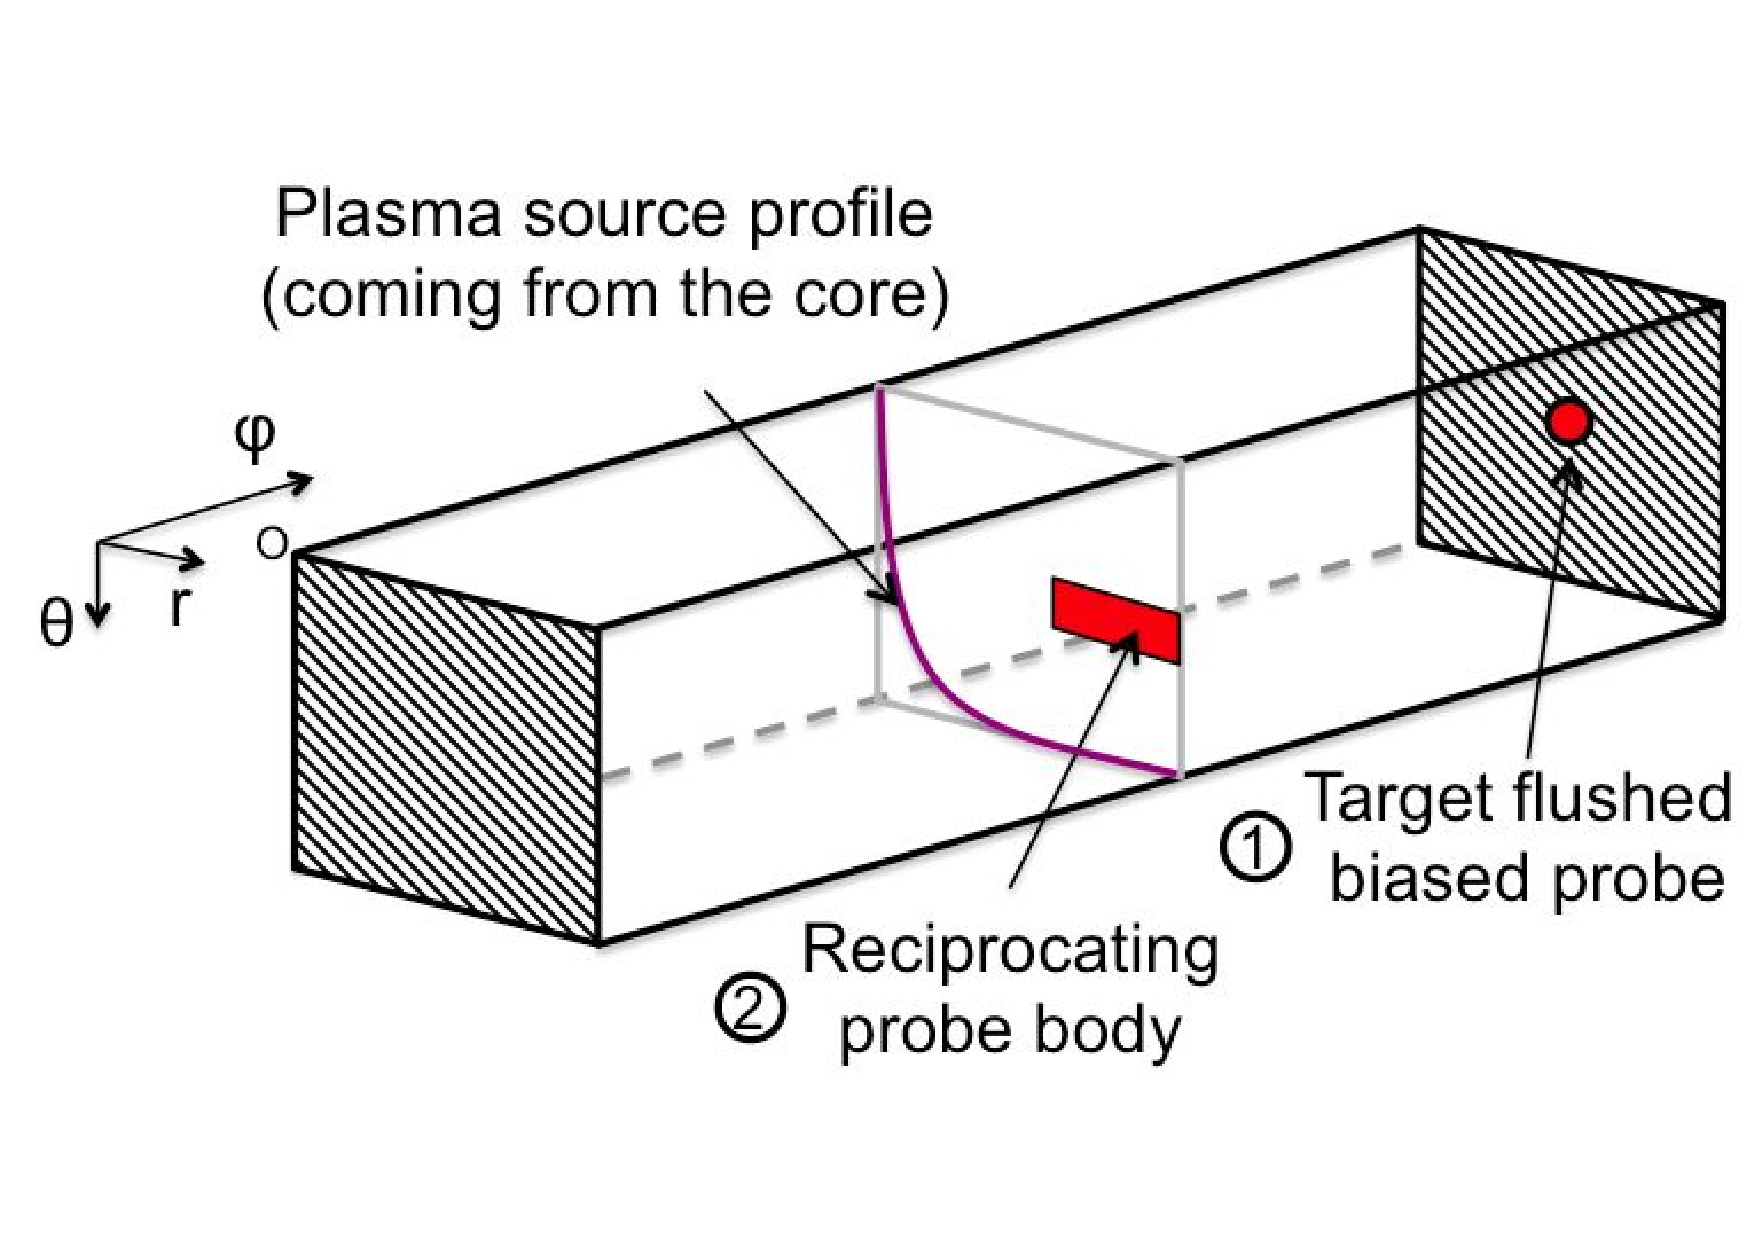
\includegraphics[width=\textwidth]{figures/geometry.pdf}
  \end{minipage}\hfill
  \begin{minipage}[c]{0.45\textwidth}
    \caption{Sketch of the slab geometry for the SOL. Divertor plates are 
 located at the end of the field lines, depicted with hatchings. The flushed
 probe is situated in the center of the top divertor plate and the mobile
 probe inserted in the middle of the domain. The
 profile of the source term driving the system is aslo roughly indicated for
 comprehension purposes.} \label{fig:1}
  \end{minipage}
\end{figure}

 The interaction between the probe
and the SOL plasma is described by the sheath theory in strong magnetic
fields, with field lines perpendicular to the wall~\cite{Bohm49}.
The flushed probe is then modeled by a local polarization of the target plates,
via a modification of the parallel Bohm boundary conditions :
 
 $$\Gamma_\parallel_\text{p}=\pm
N_\text{p}\exp(\Lambda-\Phi_\text{p}+\Phi_\text{wall})
 \qquad
 J_\parallel_\text{p} = \pm
 N_\text{p}(1-\exp(\Lambda-\Phi_\text{p}+\Phi_\text{wall}))
$$ 

$\Gamma_\parallel_\text{p}$, $N_\text{p}$,
$\Phi_\text{p}$ and $J_\parallel_\text{p}$ are plasma quantities in front of the
probe but still at the sheath entrance. The wall polarization
has a gaussian shape
$\Phi_\text{wall}=V_p\text{~}\exp(-(X-X_p)^2/L_p^2)\text{~}\exp(-(Y-Y_p)^2/L_p^2)$
with $V_p$ the applied bias voltage, $(X_p, Y_p)$ the position and $L_p$ the
size of the probe. In the limit of strong negative polarization\footnote{with a
typical SOL electronic temperature $T_0\approx$ 100 eV, $V_p=-3$ corresponds to
approximately -300V}, the Boltzmann exponential term tend toward zero locally:
only ions reach the probe and the current drawn by the probe is
equal to the ion flux, ie. the probe is run on ion saturation mode.

On the other hand, the probe body is geometrically modelled by introducting
a solid obstacle with sheath boundary condition in the middle of the plasma. The
probe covers an area of 32 $\rho_L$ in the poloidal direction and occupies
radially the second half of the computationnal zone. In the parallel
direction the probe is infinitly thin, which seems reasonnable when
considering the size of the probe in comparison to the
parallel length $L_\parallel$ of the plasma.
At least, the probe body is taken conductive, but could just as well be chosen
insulating, as we will mostly focus on density and flux perturbations.

\section{Polarisation of the divertor probe}

\subsection{\bf Macroscopic phenomology}

\begin{figure}
%\begin{wrapfigure}{l}{68mm}
%\sidecaption
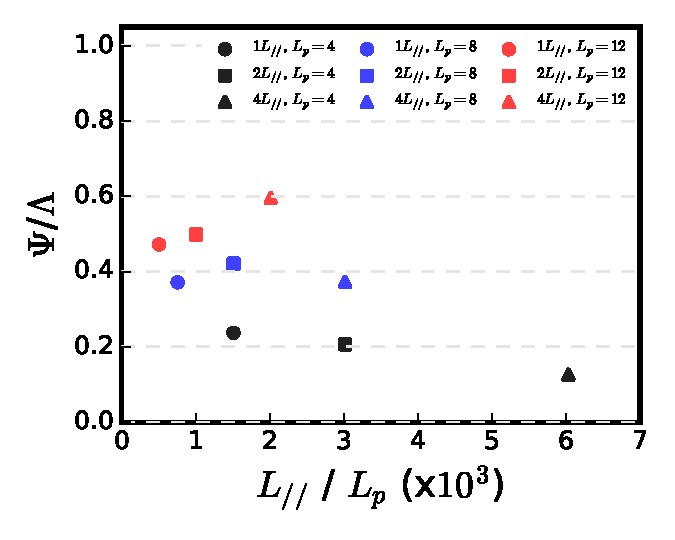
\includegraphics[width=68mm]{figures/perturbAmplLp.pdf}
\caption{Slab geometry of the SOL. The flushed probe is located at the end of
the box. The mobile probe can be situated either in the middle or at one forth
of the domain.}
\label{fig:2}
\end{figure}

 LPs
produce a polarization of the whole connected flux tube, drawing perpendicular fluxes and currents from the outside plasma. Let us now analyse the influence of
two parameters: the probe size and the probe voltage.
\begin{figure}
\begin{minipage}{68mm}
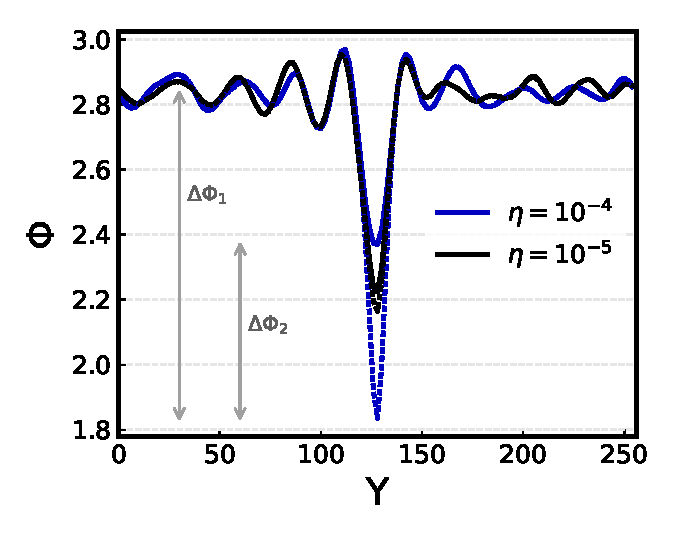
\includegraphics[width=\linewidth]{figures/poloidalProf.pdf} \caption{I-V
characteristic of the probe. Blue dashed line is the expected slope for the mean electron temperature present at
this radial location. Red thin line is the linear regression of the
characteristic between $V_p=-2$ and $V_p=1$.}
\label{fig:2}
\end{minipage}
\hfill
\begin{minipage}{68mm}
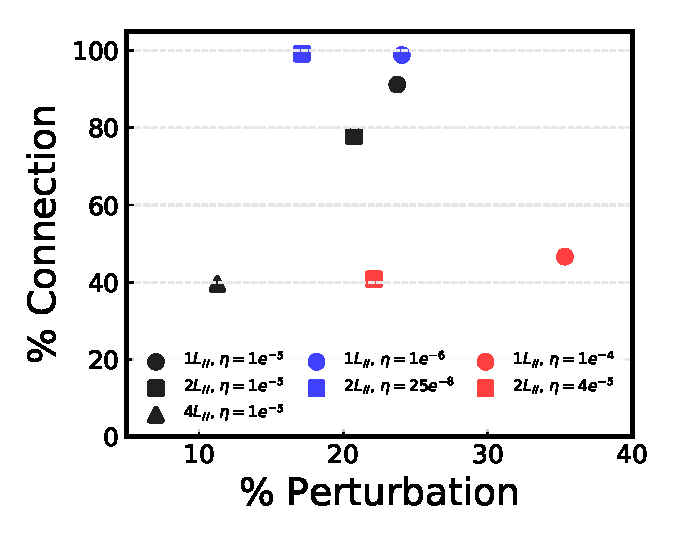
\includegraphics[width=\linewidth]{figures/perturbAmpl.pdf}
\caption{Conditionnal average of plasma fluctuations
waveforms on the poloidal direction for intermittent bursts exceeding 2 times the standard
deviation. Left axe is for $\tilde{N}$, $\tilde{\Phi}$ and $\Lambda\tilde{T}$,
right axe is for $\tilde{V}_f$.}
\label{fig:3}
\hfill
\end{minipage}
\end{figure}

\subsection{\bf 1D model}


\section{Mach probes}
The results presented in section~\ref{2D} have shown a strong perturbation of
the plasma turbulence due to the probe in a 2D reduced geometry. However,
this effect may be overestimated as with this reduction, we effectively model
two synthetic probes, one in front of each other at both ends of the field lines. In this part
we use the TOKAM3X code~\cite{Tamain15}, a 3D global edge
turbulence code based on the fluid-drift approximation, to have a look on a more
realistic 3D case where the probe is still located on the limiter, but this time on only one side of the
field line.
\subsection{\bf Perturbation the SOL plasma due to the probe body}

\subsection{\bf Synthetic Mach measurements}

\subsubsection{Measurements without parallel flow}

 
 \begin{figure}
 \begin{minipage}{60mm}
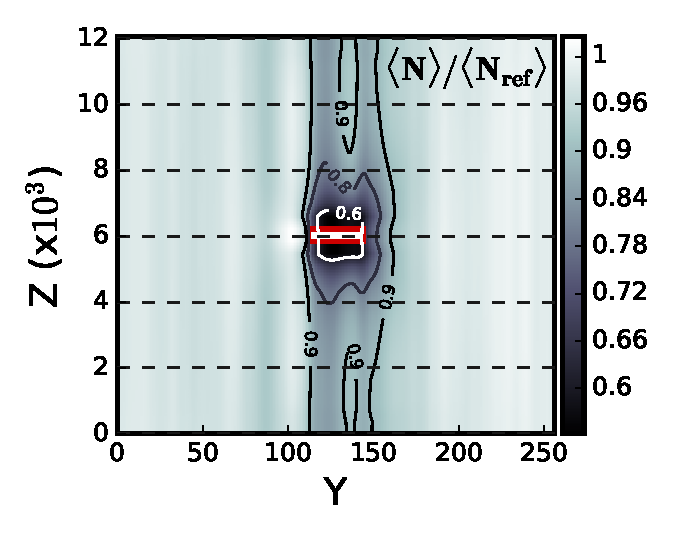
\includegraphics[width=55mm,trim = 0mm 0mm 0mm
0mm,clip]{figures/densityMapProbe.pdf}~\textbf{a)}
\end{minipage}
 \begin{minipage}{68mm}\hfill
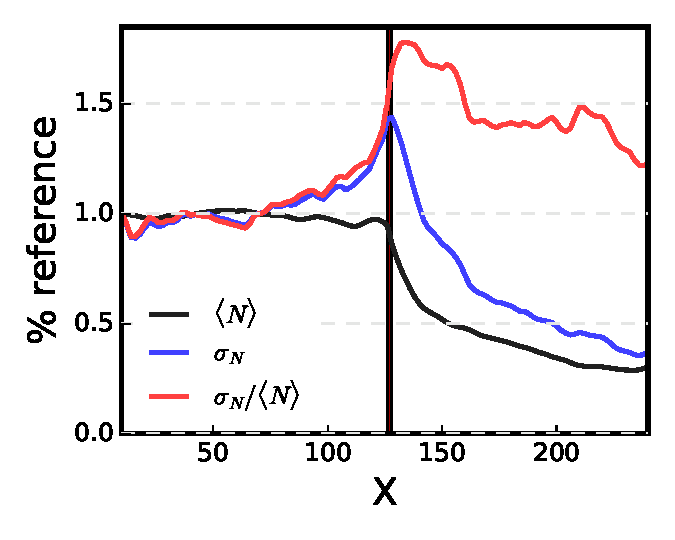
\includegraphics[width=68mm]{figures/radialProfileProbe.pdf}~\textbf{b)}
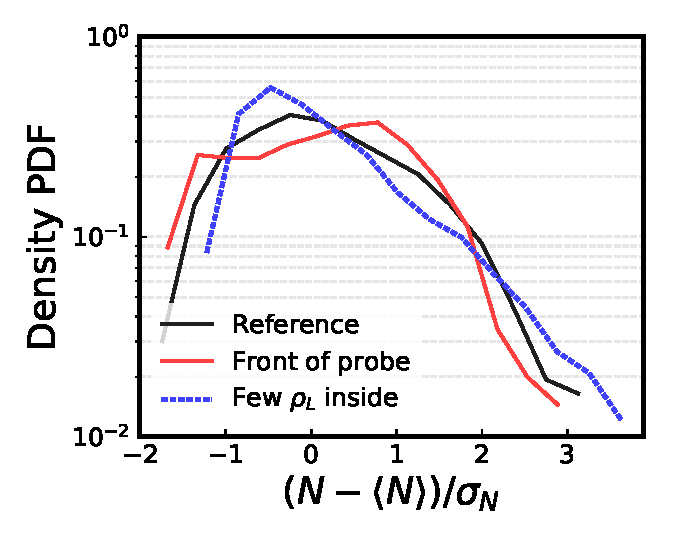
\includegraphics[width=68mm]{figures/pdfProbe.pdf}~\textbf{c)}
\label{fig:4}
\end{minipage}
\caption{\textbf{a)~} Mean density at the location of the probe. Red circles
stand for the isothermal case~\cite{Colin14} and black diamonds
for non-isothermal 2D cases. The blue square is a 3D case with probes at
each end of the field lines. Blue triangles are the 3D, one probe cases.
\textbf{b)}~Ratio of difference between the parallel current drawn by the probe
$J_{\parallel p}$ and the current coming from the opposite wall
$J_{\parallel o}$ as a function
of the parallel length and for different probe sizes.}
\end{figure}

\subsubsection{Measurements in the presence of parallel flow}

 
\section{Discussion}

\section{Conclusion}
% When the probe draws a current, some part has to come from the perpendicular
% direction\footnote{If the probe draws no current from the perpendicular
% direction, $\nabla_\parallel j_\parallel$ should be null, and thus $j_\parallel$
% a constant. The Bohm sheath conditions impose then $V_p=0$, and a zero parallel
% current as well.}. Let's assume a simple diffusive/viscous process controled by
% $\nu^*$.
% The charge balance equation gives
% 	$\nabla_\parallel j_\parallel=\nabla_\perp\cdot\nu^*\nabla_\perp\nabla_\perp^2
% 	\Phi$. If we suppose a mean perturbation on the potential of size $L_s$, the
% 	current equilibrium of the 2D model is then :
% 	\begin{gather}
% 	\sigma_\parallel(\Lambda-(\Phi-V_p)/T_p)=(\Phi-\Lambda
% 	T)\nu^*/L_s^2L_\perp^2\Longleftrightarrow\Phi\approx\frac{1}{1+r}\left(V_p-\Lambda\left(T+rT_p\right)
% 	\right)
% 	\end{gather}
% with $r=\nu /L_s^2L_\perp^2\sigma_\parallel$ a transport ratio. As $r\propto
% L_S^{-2}$, when the probe size increase, the plasma potential will adapt to the wall sheath
% potential $V_p-\Lambda T_p$, $T_p$ being the electronic temperature at the probe
% location. In contrast, for a small probe size of when the perpendicular
% transport is efficient, the plasma potential will go as the unperturbed plasma
% sheath potential $\Phi=\Lambda T$. The same work for the 3D case give , 


\begin{acknowledgement}
This work has been financialy supported by the French National Research
Agency through project ANR-11-BS09-023 (SEDIBA). It has been carried out within
the framework of the EUROfusion Consortium with a funding from the
Euratom research and training programme 2014-2018 in the frame of project
WP14-ER-01/CEA-09. The views and opinions expressed herein do not necessarily
reflect those of the European Commission. This work was granted access to the
HPC resources of Aix-Marseille Universit� financed by the project Equip@Meso
(ANR-10-EQPX-29-01) of the programme "Investissements d'Avenir" supervised by
the Agence Nationale pour la Recherche. It also used HPC resources from
GENCI-IDRIS in the frame of project i2015056912.
\end{acknowledgement}


\def\bstname{cpp}

 \bibliographystyle{cpp}
 \bibliography{biblio.bib}
% 
% Replace the following example bibliography with your references
% before submission:
%\providecommand{\WileyBibTextsc}{}
%\let\textsc\WileyBibTextsc
%\providecommand{\othercit}{}
%\providecommand{\jr}[1]{#1}
%\providecommand{\etal}{~et~al.}


%\begin{thebibliography}{[10]}


%\end{thebibliography}


\end{document}
